\chapter{Planning}
\section{Risk analysis}
There are several risks in the project. The first risk is hard to estimate the time of the model and rigging due to lack of relevant experience. So initially to tackle this problem, a spider model will be found on the Internet. The biggest risk is to implement the three layers in\cite{steering} which is usually implemented under the physical modeling. The second biggest risk is the inverse kinematics may not produce the expected results or is hard to be embedded in the system due to lack of experience. The fall-back schema is to implement a behavior-stepping pairs instead of implementing the three layers. About the animation techniques, if the expected results or the skeleton animation is too hard to implement, scene graph techniques along with procedural animation or keyframe animation will be adopted. The results of adopting backup plan is that the animation results will not be good as expected and as a result of changing plan, some requirements listed in Chapter 3 may not be fully satisfied.
There are also risks that there not enough volunteers to judge the project. Two possible solutions to it is that invite the volunteers before the poster session and evaluate the project against videos of real spider which does not require many volunteers. 
If the results of the project are not ready on time for the evaluation stage, efforts in the project should be ready to be demonstrated either under Oculus Rift or using a PC. As a result, work in each stages should be recorded to prepare for this kind risk. 
There are also some risks which can not be foreseen at this stage. So contingency time along with some risks mentioned above should be considered in project plan.
\section{Project plan}
The project plan is based on the analysis in Chapter 3. Figure \ref{fig:gantTable} and figure \ref{fig:gant} are Gantt table and chart. 
\begin{figure}[ht!]
\centering
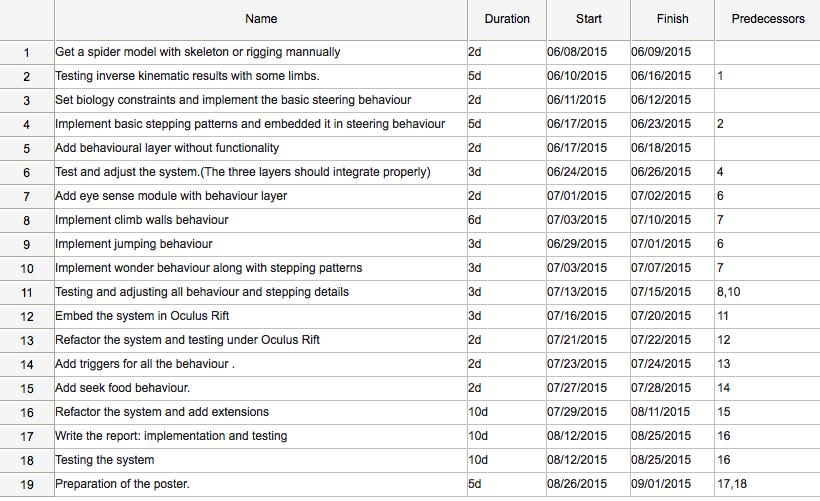
\includegraphics[width=15cm]{figures/gantTable.png}
\caption{Gantt Table}
\label{fig:gantTable}
\end{figure}
\begin{figure}[ht!]
\centering
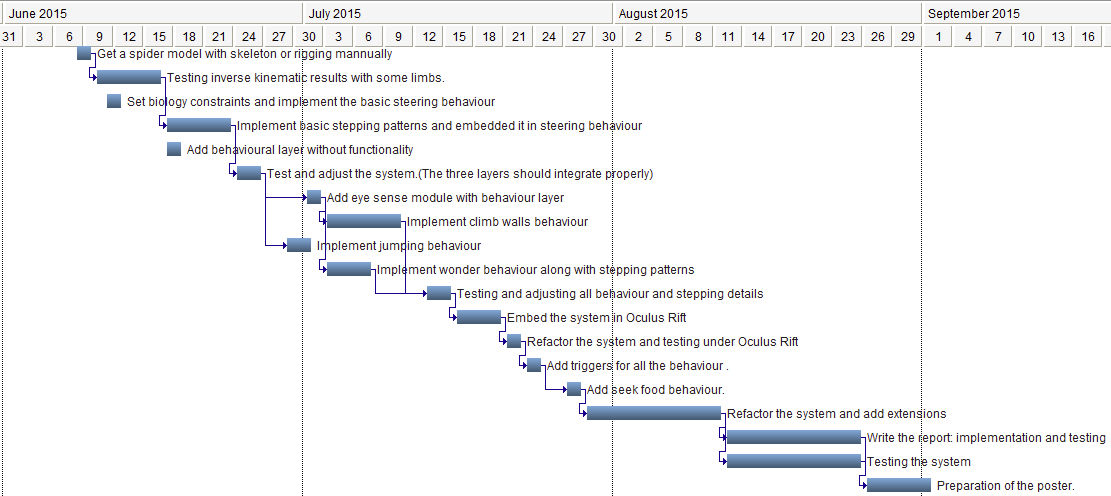
\includegraphics[width=15cm]{figures/gant.png}
\caption{Gantt Chart}
\label{fig:gant}
\end{figure}
All tasks in the figure are assigned more time than the amount that they can be finished in. About the animation techniques may be different than as planned, the task 2 "Testing inverse kinematics..." is testing whether the technique is suitable. So the animation technique could be chosen properly in the early stage and the techniques will not interfere with the following tasks. About the risk that the main schema may not work, the plan is added system prototype testing and adjusting stage. Besides, the system will not implement the main schema such as three layers in \cite{steering} at early stage, it will implement several subtasks which is not dependent on the main schema. The main schema will be added in later stage to avoid much dependancy. 
